\documentclass{../template/Report}%方括号内写yuxi即生成预习报告\documentclass[yuxi]{../template/Report}
\settemplatedir{../template/}%设置模板路径

\exname{} %实验名称
\extable{} %实验桌号
\instructor{} %指导教师
\class{} %班级
\name{} %姓名
\stuid{} %学号

\nyear{} %年
\nmonth{} %月
\nday{} %日
\nweekday{} %星期几，e.g. \nweekday{三}
\daypart{}%上午/下午

\redate{} %如有实验补做，补做日期
\resitu{} %情况说明：

\begin{document}
\maketitle%输出封面

\section{预习报告（10分）}

\subsection{实验综述（5分）}

\subsubsection{实验原理}

\paragraph{载流圆线圈与亥姆霍兹线圈的磁场分布}
本实验旨在研究不同线圈组合下的磁场分布特性。
对于半径为 $R$、匝数为 $N_0$ 的载流圆线圈，当通以直流电流 $I$ 时，根据毕奥-萨伐尔定律，其轴线上距离圆心 $X$ 处的磁感应强度 $B$ 可表示为：
\begin{equation}
    B = \frac{\mu_0 N_0 I R^2}{2 (R^2 + X^2)^{3/2}}
\end{equation}
式中 $\mu_0$ 为真空磁导率。理论上，单一线圈的磁场分布呈单峰状，以线圈中心为对称轴向两侧衰减。

为了获得均匀磁场，通常采用亥姆霍兹线圈结构。如\cref{fig:xianquan}右图所示，该装置由两个完全相同的圆线圈组成，它们彼此平行、共轴，且通以同向电流。当两线圈间距 $d$ 严格等于线圈半径 $R$ 时，两线圈产生的磁场在中心区域相互叠加，使得中心轴线附近较大范围内形成均匀度极高的匀强磁场区。

\begin{figure}[H]
    \centering
    
\includegraphics[width=0.7\textwidth]{figues/huoerfa/xianquan.png}
    \caption{载流圆线圈（左）与亥姆霍兹线圈（右）的磁场分布示意图}
    \label{fig:xianquan}
\end{figure}

\paragraph{霍尔效应测量原理}
本实验利用霍尔效应来探测上述磁场分布。霍尔效应是指置于磁场中的载流导体，在垂直于电流和磁场的方向上产生电势差的现象。
如\cref{fig:huoerxiaoying}所示，设霍尔元件为 $P$ 型半导体，厚度为 $d$。当工作电流 $I_H$ 流过元件，且磁场 $B$ 垂直作用于薄片表面时，载流子（空穴）在洛伦兹力 $F_B = q(\boldsymbol{v} \times \boldsymbol{B})$ 的作用下发生横向偏转，并在元件两侧（$a, b$ 面）积累电荷。
这种电荷积累建立了横向电场 $E$，当电场力 $F_E = qE$ 与洛伦兹力达到动态平衡时，两侧电势差趋于稳定，该电势差称为霍尔电压 $U_H$。

\begin{figure}[H]
    \centering
    
\includegraphics[width=0.5\textwidth]{figues/huoerfa/huoerxiaoying.png}
    \caption{利用霍尔效应测磁场的原理图}
    \label{fig:huoerxiaoying}
\end{figure}

霍尔电压与磁感应强度遵循如下线性关系：
\begin{equation}
    U_H = K_H \cdot I_H \cdot B
\end{equation}
式中 $K_H$ 为霍尔元件的灵敏度，其单位通常表示为 \unit{\milli\volt\per\milli\ampere\per\tesla}。在已知灵敏度 $K_H$ 和工作电流 $I_H$的前提下，通过测量霍尔电压 $U_H$，即可反解出待测磁场 $B$ 的大小。

\subsubsection{实验内容与预期现象}
实验将围绕磁场分布的测量与分析展开。首先测量单个载流圆线圈轴线上的磁场，预期观测到磁感应强度 $B$ 随距离 $X$ 呈钟形分布，且关于圆心严格对称。

随后构建亥姆霍兹线圈，测量其轴线磁场。当线圈间距 $d=R$ 时，预期在两线圈中心连线区域观测到一段 $B$ 值基本恒定的“平台期”，即匀强磁场区。在此基础上，进一步改变线圈间距（设置为 $d=R/2$ 或 $d=2R$），对比不同间距下磁场分布的均匀性变化，验证亥姆霍兹条件的唯一性。

此外，实验还将探索载流圆线圈沿径向的磁场分布规律，以建立对空间磁场分布的立体认知。

\subsection{实验重点（3分）}
\begin{enumerate}
    \item \textbf{原理掌握与仪器使用}：深入理解霍尔效应的物理机制，熟练掌握FB511型霍尔法亥姆霍兹线圈磁场实验仪的操作，包括励磁电流的调节与读数。
    \item \textbf{轴向磁场分布测量}：通过移动霍尔传感器，精确描绘载流圆线圈及亥姆霍兹线圈轴线上的磁场分布曲线，验证理论公式。
    \item \textbf{间距对磁场均匀性的影响}：通过对比 $d=R$、$d=R/2$ 及 $d=2R$ 三种情形下的磁场分布，量化分析线圈间距对磁场均匀区范围的影响。
\end{enumerate}

\subsection{实验难点（2分）}
\begin{enumerate}
    \item \textbf{系统误差的消除}：霍尔元件测量中存在“不等位电势”等副效应干扰。难点在于如何通过改变工作电流方向和磁场方向（对称测量法）来有效消除地磁场、热电势及不等位电势引入的系统误差。
    \item \textbf{实验操作的精准度}：传感器探头位置的微小偏差都会显著影响测量结果，特别是在测量径向分布或寻找亥姆霍兹线圈中心点时，需精细控制探头位移。
    \item \textbf{数据处理与参数计算}：需要结合霍尔元件的具体参数（如灵敏度 $K_H$）进行计算，并正确处理单位换算，将电压读数准确映射为磁感应强度。
\end{enumerate}

\begin{fullreportonly}
    \section{原始数据（20分）}
    % 此处请粘贴您的原始数据图片
    \section{结果与分析（60分）}
    \subsection{数据处理与结果（30分）}

    \subsubsection{地磁场测量}
    根据测量数据，地磁场大小记录如下（单位：\unit{\micro\tesla}）：
    \begin{equation*}
        22, 21, 24, 23, 24, 24, 26, 25
    \end{equation*}

    \paragraph{平均值计算}：

    为了保持精度与被测物理量一致，取平均值为：

    \begin{equation*}
        \bar{B}_{\text{earth}} = \SI{24}{\micro\tesla}
    \end{equation*}

    \paragraph{A类不确定度计算}：

    计算标准偏差 $S$：

    \begin{equation*}
        S = \sqrt{\frac{\sum(B_i - \bar{B})^2}{n-1}} \approx \SI{1.60}{\micro\tesla}
    \end{equation*}

    平均值的标准不确定度 $u_A$：

    \begin{equation*}
        u_A = \frac{S}{\sqrt{n}} = \frac{1.60}{\sqrt{8}} \approx \SI{1}{\micro\tesla}
    \end{equation*}

    故地磁场测量结果表示为：$B_{\text{earth}} = \SI{24(1)}{\micro\tesla}$。

    \subsubsection{单线圈磁场分布}

    实验参数：匝数 $N=400$，电流 $I=\SI{0.400}{A}$，半径 $R=\SI{0.100}{m}$。

    理论公式：

    \begin{equation*}
        B = \frac{\mu_0 N I R^2}{2(R^2 + x^2)^{3/2}}
    \end{equation*}
    其中 $\mu_0 = 4\pi \times 10^{-7} \ \si{T\cdot m/A}$。

    单线圈轴线上磁感应强度测量数据与理论值对比如表 \ref{tab:single_coil} 所示。
    其中 $B_{\text{avg}} = (|B_{\text{pos}}| + |B_{\text{neg}}|)/2$。

    \begin{table}[H]
        \centering
        \caption{单线圈通电圆线圈磁场分布测量数据与理论值对比}
        \label{tab:single_coil}
        \small
        \begin{tabular}{c c c c c c c}
            \toprule
            \textbf{位置} $x$ & \textbf{位置} $S$ & $B_{\text{正}}$      & $B_{\text{负}}$      & $B_{\text{平均}}$     & $B_{\text{理论}}$     & \textbf{相对误差} \\
            (\si{cm})       & (\si{cm})       & (\si{\micro\tesla}) & (\si{\micro\tesla}) & (\si{\micro\tesla}) & (\si{\micro\tesla}) & (\%)          \\
            \midrule
            -10.00          & 5.00            & 359                 & -363                & 361.0               & 355.4               & 1.57          \\
            -9.00           & 6.00            & 413                 & -424                & 418.5               & 412.8               & 1.37          \\
            -8.00           & 7.00            & 479                 & -488                & 483.5               & 478.7               & 1.01          \\
            -7.00           & 8.00            & 554                 & -563                & 558.5               & 552.7               & 1.04          \\
            -6.00           & 9.00            & 635                 & -642                & 638.5               & 633.9               & 0.73          \\
            -5.00           & 10.00           & 716                 & -734                & 725.0               & 719.3               & 0.79          \\
            -4.00           & 11.00           & 804                 & -814                & 809.0               & 804.7               & 0.54          \\
            -3.00           & 12.00           & 887                 & -889                & 888.0               & 883.4               & 0.52          \\
            -2.00           & 13.00           & 949                 & -947                & 948.0               & 947.9               & 0.01          \\
            -1.00           & 14.00           & 988                 & -994                & 991.0               & 990.4               & 0.06          \\
            0.00            & 15.00           & 994                 & -1004               & 999.0               & 1005.3              & 0.63          \\
            1.00            & 16.00           & 974                 & -990                & 982.0               & 990.4               & 0.85          \\
            2.00            & 17.00           & 936                 & -944                & 940.0               & 947.9               & 0.83          \\
            3.00            & 18.00           & 869                 & -879                & 874.0               & 883.4               & 1.06          \\
            4.00            & 19.00           & 790                 & -804                & 797.0               & 804.7               & 0.95          \\
            5.00            & 20.00           & 706                 & -717                & 711.5               & 719.3               & 1.09          \\
            6.00            & 21.00           & 620                 & -638                & 629.0               & 633.9               & 0.77          \\
            7.00            & 22.00           & 537                 & -558                & 547.5               & 552.7               & 0.95          \\
            8.00            & 23.00           & 464                 & -488                & 476.0               & 478.7               & 0.56          \\
            9.00            & 24.00           & 402                 & -416                & 409.0               & 412.8               & 0.93          \\
            10.00           & 25.00           & 344                 & -360                & 352.0               & 355.4               & 0.97          \\
            \bottomrule
        \end{tabular}
    \end{table}

    \paragraph{绘制$B - x$曲线}

    \begin{figure}[H]
        \centering
        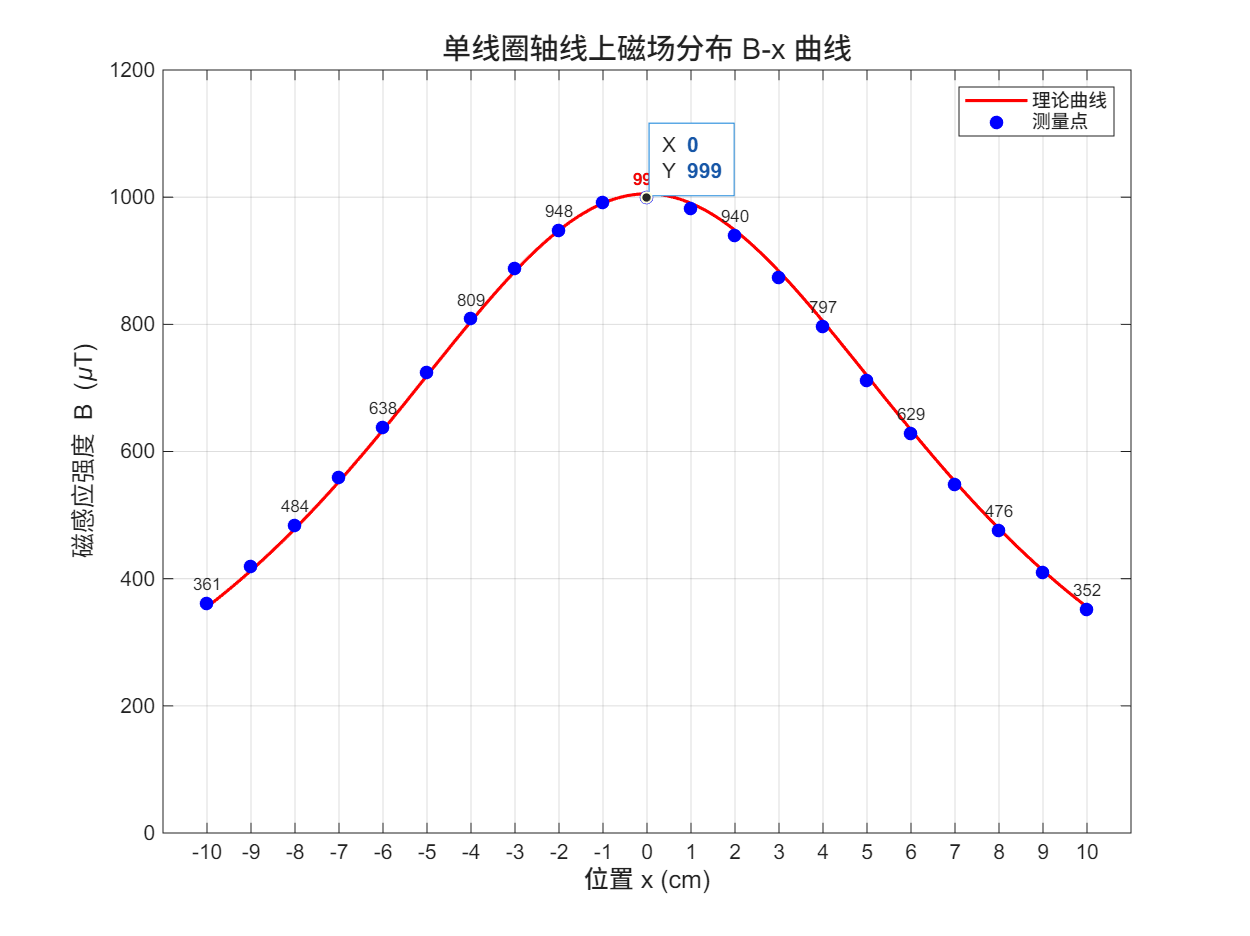
\includegraphics[width = .8\textwidth]{./figures/单线圈.png}
        \caption{单线圈磁场分布曲线}
        \label{fig:single_coil}
    \end{figure}

    \paragraph{曲线特性分析}：
    如\cref{fig:single_coil}所示，单线圈轴线上的磁场分布呈现中间高、两端低的钟形分布。
    在圆心处（$x=0$）磁感应强度最大，随着距离 $|x|$ 的增加，磁场逐渐减小。
    实验测量曲线与理论计算曲线吻合度较好，尤其在中心区域误差极小。

    \subsubsection{亥姆霍兹线圈磁场分布}
    亥姆霍兹线圈由两个相同的线圈共轴放置，间距等于半径 $R=\SI{0.100}{\meter}$。

    中心点磁感应强度的理论值计算：
    \begin{equation*}
        B_{\text{theory}} = \left(\frac{4}{5}\right)^{3/2} \frac{\mu_0 N I}{R} = 0.7155 \times \frac{4\pi \times 10^{-7} \times 400 \times 0.4}{0.1} \approx \SI{1438.7}{\micro\tesla}
    \end{equation*}

    测量数据及中心点误差如\cref{tab:hmhz}所示：

    \begin{table}[H]
        \centering
        \caption{亥姆霍兹线圈磁场分布测量数据}
        \label{tab:hmhz}
        \small
        \begin{tabular}{c c c c c}
            \toprule
            \textbf{位置} $x$ (\si{cm}) & $B_{\text{正}}$ (\si{\micro\tesla}) & $B_{\text{负}}$ (\si{\micro\tesla}) & $B_{\text{平均}}$ (\si{\micro\tesla}) & \textbf{备注}  \\
            \midrule
            -10.00                    & 890                                & -884                               & 887.0                               &              \\
            -9.00                     & 1006                               & -994                               & 1000.0                              &              \\
            -8.00                     & 1111                               & -1105                              & 1108.0                              &              \\
            -7.00                     & 1210                               & -1202                              & 1206.0                              &              \\
            -6.00                     & 1293                               & -1281                              & 1287.0                              &              \\
            -5.00                     & 1359                               & -1344                              & 1351.5                              &              \\
            -4.00                     & 1400                               & -1386                              & 1393.0                              &              \\
            -3.00                     & 1422                               & -1408                              & 1415.0                              &              \\
            -2.00                     & 1426                               & -1416                              & 1421.0                              &              \\
            -1.00                     & 1431                               & -1417                              & 1424.0                              &              \\
            0.00                      & 1438                               & -1410                              & 1424.0                              & \textbf{中心点} \\
            1.00                      & 1433                               & -1414                              & 1423.5                              &              \\
            2.00                      & 1436                               & -1406                              & 1421.0                              &              \\
            3.00                      & 1431                               & -1397                              & 1414.0                              &              \\
            4.00                      & 1402                               & -1382                              & 1392.0                              &              \\
            5.00                      & 1370                               & -1340                              & 1355.0                              &              \\
            6.00                      & 1310                               & -1276                              & 1293.0                              &              \\
            7.00                      & 1226                               & -1200                              & 1213.0                              &              \\
            8.00                      & 1132                               & -1106                              & 1119.0                              &              \\
            9.00                      & 1030                               & -990                               & 1010.0                              &              \\
            10.00                     & 925                                & -878                               & 901.5                               &              \\
            \bottomrule
        \end{tabular}
    \end{table}

    \paragraph{绘制亥姆霍兹线圈的$B - x$曲线}
    \begin{figure}[H]
        \centering
        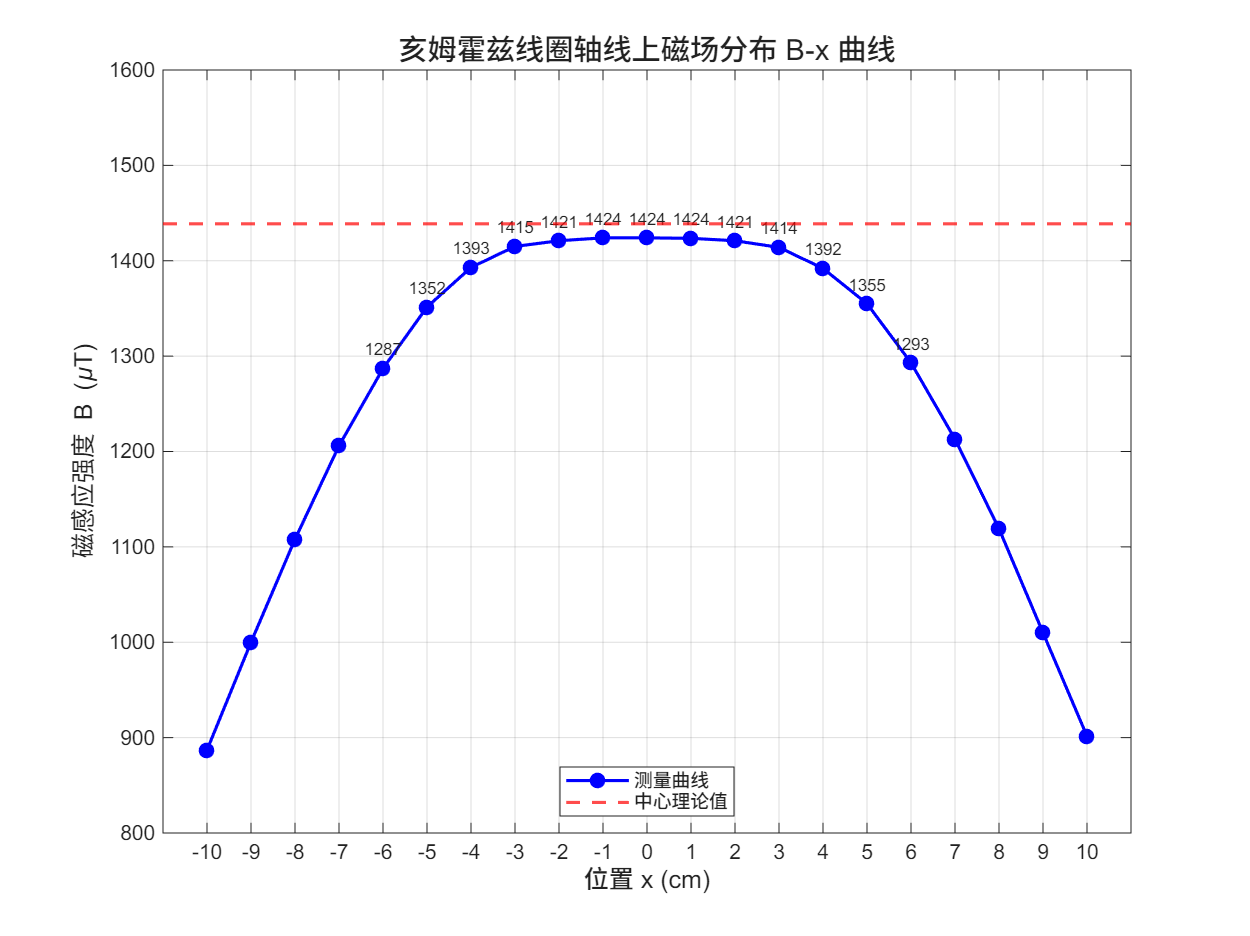
\includegraphics[width = .8\textwidth]{./figures/亥姆霍兹.png}
        \caption{亥姆霍兹线圈磁场分布曲线}
        \label{fig:hmhz}
    \end{figure}

    \paragraph{曲线特性分析}：
    如\cref{fig:hmhz}所示，亥姆霍兹线圈在两线圈中心附近（$x=0$ 附近）产生了一个较宽的均匀磁场区。
    与单线圈相比，其磁场变化在中心区域更加平缓，验证了亥姆霍兹线圈产生均匀磁场的特性。

    中心点磁感应强度的理论值计算：
    \begin{equation*}
        B_{\text{theory}} = \left(\frac{4}{5}\right)^{3/2} \frac{\mu_0 N I}{R} = 0.7155 \times \frac{4\pi \times 10^{-7} \times 400 \times 0.4}{0.1} \approx \SI{1438.7}{\micro\tesla}
    \end{equation*}

    \paragraph{中心点误差计算}：
    \begin{equation*}
        E = \frac{|B_{\text{meas}} - B_{\text{theory}}|}{B_{\text{theory}}} \times 100\% = \frac{|1424.0 - 1438.7|}{1438.7} \times 100\% \approx 1.02\%
    \end{equation*}

    \subsection{误差分析（20分）}
    \begin{enumerate}
        \item \textbf{相对误差分析}：单线圈中心点的测量相对误差为 $0.63\%$，亥姆霍兹线圈中心点的相对误差为 $1.02\%$。
              误差来源可能包括：霍尔传感器的位置未能精确对准线圈几何中心；
              线圈匝数或半径的标称值与实际值存在微小偏差；地磁场未完全消除或读数时的零点漂移。
        \item \textbf{坐标定位误差}：由于移动传感器时标尺读数存在视差，
              或者传感器探头在移动过程中发生了微小的角度偏转，导致测量值偏离理论值。
    \end{enumerate}
    \subsection{实验探讨（10分）}
    本实验成功验证了载流圆线圈和亥姆霍兹线圈的磁场分布特性。
    霍尔效应法测磁场灵敏度高，但对位置和角度较为敏感。
    实验发现亥姆霍兹线圈在中心区域提供了非常均匀的磁场环境，
    这在需要均匀磁场的科学研究和工业应用中具有重要意义。

    \section{思考题（10分）}

    \subsection{为什么在测量直流磁场时，必须考虑地球磁场对被测磁场的影响？}
    因为地球磁场是一个矢量，存在于任何实验环境中（大小约为 $\SI{50}{\micro\tesla}$ 量级）。
    根据磁场叠加原理，霍尔传感器测得的实际磁场 $\vec{B}_{\text{meas}}$ 是线圈产生的磁场 $\vec{B}_{\text{coil}}$ 与地磁场 $\vec{B}_{\text{earth}}$ 的矢量和。

    当被测磁场较弱时，地磁场的分量可能与被测磁场量级相当，若不消除其影响，会造成显著的系统误差。

    但是在实验中，通常采用改变电流方向测量两次（$B_+, B_-$）并平均 $B = (|B_+| + |B_-|)/2$ 来消除地磁场及零点漂移的影响。

    \subsection{载流圆线圈轴线上磁场的分布规律如何？}
    磁场分布具有对称性，它关于线圈圆心（$x=0$）呈轴对称分布，而且在圆心处，磁感应强度取到最大值。

    随着距离圆心 $|x|$ 的增大，磁感应强度 $B$ 单调递减。在圆心附近变化较慢，随着距离增加衰减速度加快，呈现出钟形的分布特征。

    \subsection{亥姆霍兹线圈是怎样组成的？其基本条件有哪些？它的磁场分布特点又怎样？改变线圈间距后，线圈轴线上的磁场分布情况如何？}
    \begin{enumerate}
        \item \textbf{组成与条件}：亥姆霍兹线圈由两个半径 $R$ 相同、匝数 $N$ 相同、彼此平行的同轴圆线圈组成。基本条件是两个线圈串联通以同向、大小相等的电流 $I$，且两线圈之间的距离 $d$ 严格等于线圈半径 $R$。
        \item \textbf{磁场分布特点}：在两线圈中心 $O$ 点附近，磁场的一阶导数 $\frac{\textrm{d}B}{\textrm{d}x}$ 和二阶导数 $\frac{\textrm{d}^2B}{\textrm{d}x^2}$ 均为零，形成一个较宽的均匀磁场区域。
        \item \textbf{改变间距的影响}：
              \begin{enumerate}
                  \item 当 $d < R$ 时：中心点 $O$ 处出现极小值，两侧各有一个极大值，磁场呈双峰状。
                  \item 当 $d > R$ 时：中心点 $O$ 处虽仍是极大值，但磁场随距离增加而急剧下降，均匀区变窄。
                  \item 只有当 $d = R$ 时，叠加后的磁场最平坦，均匀度最好。
              \end{enumerate}
    \end{enumerate}

    \subsection{霍尔元件放入磁场时，不同方向上的特斯拉计指示值不同，哪个方向最大？}
    答：当霍尔元件的工作平面与磁感应强度矢量 $\vec{B}$ 的方向\textbf{垂直}时，穿过元件的磁通量最大，霍尔电压 $V_H$ 达到最大值，此时特斯拉计的指示值最大。

    \subsection{试分析载流圆线圈磁场分布的理论值和实际值的误差产生的原因？}
    该实验可能存在系统误差，如地磁场未能通过换向完全消除；霍尔传感器存在零点漂移或非线性误差；线圈的实际半径 $R$ 和匝数 $N$ 与标称值存在偏差。

    操作中可能引入人为误差，探头位置调节不准，霍尔元件中心未严格处于线圈轴线上；移动坐标 $x$ 时读数视差或标尺精度限制；探头方向未严格垂直于磁场方向。

    实验室环境也有影响，如周围铁磁性物质或其它电气设备的杂散磁场干扰。
\end{fullreportonly}
\insertnotes
\end{document}